
\section{New Energy-Aware Scheduling Algorithms} \label{sec:algorithms}

As a means of producing fewer energy violations and in the meantime meeting the task deadlines when scheduling system tasks, we have developed two techniques that work effectively without depending on energy predication: the \emph{Smooth to Average Method} (\textsc{STAM}) and the \emph{Smooth to Full Utilization} (\textsc{STFU}). 

\subsection{Smooth to Average Method}
First we illustrate a core concept, \emph{virtual tasks}, used in our methods.

\begin{definition}
Given a task $\tau = <I, T, E>$ and an energy threshold value $\bar{E}$, its equivalent \emph{virtual task} is defined as the task $\bar{\tau} = <I, \lceil T *  E/\bar{E} \rceil, \bar{E}>$.
\end{definition}

To distinguish, we call the real task $\tau$ a \emph{physical task} in the rest of the paper.

\begin{remark}
When the energy threshold value $\bar{E}$ is larger than $E$, the task $\tau$ is the same as the task $\bar{\tau}$. When the energy threshold value $\bar{E}$ is not larger than $E$, task $\tau$ and the virtual task $\bar{\tau}$ will consume roughly the same amount of energy. It is easy to see that the virtual task $\bar{\tau}$ will require longer execution time than task $\tau$ in this case, and as such any scheduling algorithm that can schedule the virtual task without violating its deadline constraint will meet the deadline for the physical task as well. 
\end{remark}
\begin{remark}
The motivation of introducing virtual tasks is to smooth the energy consumption in the long run. If we make a schedule using the virtual tasks, but actually execute the physical tasks according to the schedule, the consequence is that the system will automatically wait for energy replenishment before running a request that consumes a large amount of energy. The waiting time is proportional to the energy amount consumed by the request.
\end{remark}

Intuitively, it would be a good choice to smooth the energy consumption to the average energy requirement per unit time of all tasks in a given task list. The STAM is designed for such a purpose. We generate a set of equivalent \emph{virtual tasks} by increasing the duration of any task that uses greater than average energy per unit time, thus \emph{smoothing} each task to approximately the average energy per time unit. In these virtual tasks, the total energy remains the same as that in the real tasks, but it is spread over a longer duration.  Virtual tasks cannot be scheduled to run at the same time and are not preemptible.  Once the virtual tasks are scheduled, the physical tasks are inserted at the end of the corresponding virtual task's timeslot.  Thus a physical task that consumes high energy is guaranteed to run after an idle period, which reduces the likelihood that the system will run out of energy when the task runs. 

\begin{algorithm}[htb]
\label{stamalg}
\begin{algorithmic}
\STATE INPUT: $realTasks$ \COMMENT {list of [period, duration, energy]} 
\STATE INPUT: $N$ \COMMENT {number of tasks}
\STATE OUTPUT: $vTasks$ \COMMENT {same format as $realTasks$}
\STATE $E_{mean} \gets mean(realTasks[:,3])$
\FOR{$i = 1$ \TO $N$}
\IF{$taskList[i,3] > E_{mean}$}
\STATE $E_i \gets realTasks[i, 2] \times realTasks[i,3]$
\STATE $D_V \gets \lceil \frac{E_i}{E_{mean}} \rceil$
\STATE $E_V \gets \frac{E_i}{D_V}$
\STATE $vTasks[i,:] \gets [taskList[i,1]~~D_V~~E_V]$
\ELSE
\STATE $vTasks[i,:] \gets taskList[i,:]$
\ENDIF
\ENDFOR
\end{algorithmic}
\caption{Generate \textsc{STAM} Task List}
\end{algorithm}

The \textsc{STAM} algorithm calculates the energy consumption of each task by multiplying its runtime by the task's energy consumption per time unit. After taking the mean energy consumption across all of the tasks in the task list, each task is compared to the this value and virtual tasks are generated accordingly. If the given task's energy consumption is above the mean energy value, the virtual duration is calculated by taking the ceiling of the energy area of the task divided by the calculated energy mean. This will extend the duration of the virtual task allowing the total energy consumed to be more evenly distributed across the duration of the task's runtime. If the given task's energy consumption is below the calculated energy mean, the algorithm is unable to perform any smoothing and  will use the unchanged physical task to generate a schedule.

\subsection{Smooth to Full Utilization}

A potential problem of STAM is that the virtual tasks may be spread across too long a duration such that no scheduling is possible to meet the deadline constraints of the virtual tasks. This may happen if some physical tasks require very high energy amount and thus the corresponding virtual tasks enforce the system to wait for a long time. To avoid this problem, we propose a different heuristic to smooth the energy consumption, called \emph{Smooth to Full Utilization} (\textsc{STFU}).  

The \textsc{STFU} algorithm is similar to STAM, but instead of smoothing all tasks to the average energy usage, \textsc{STFU} attempts to create a virtual task list with 100\% \emph{virtual utilization}\footnote{The CPU utilization calculated based on virtual tasks is called virtual utilization.}, $U_V$.  In other words, in a schedule generated from a virtual task list output by \textsc{STFU}, the likelihood of there being a virtual task scheduled at any arbitrary time is as close as possible to 100\%.

Utilization $U$ is defined in equation~\ref{eqn:utilization}, where $k$ is the number of tasks, $D_i$ is the duration of the $i^{th}$ task, and $P_i$ is the period of the $i^{th}$ task.
\begin{equation}
\label{eqn:utilization}
U = \sum_{i=1}^{k} \frac{D_i}{P_i}
\end{equation}

\nop{As $U \to 100\%$, EDF becomes the optimal scheduling algorithm regardless of energy. [nrqm - is this correct?]}

To generate a virtual task list with STFU, first each task is given a virtual duty cycle $d_V$ representing what proportion of the total run time will be allocated to the corresponding virtual task.  The goal of STFU is to allocate more time to tasks that use greater energy, so that a high-energy task has more time to harvest energy before executing.  A task that uses $40\%$ of the total energy consumed by tasks should be given a virtual duty cycle of $d=40\%$.  Virtual tasks cannot have a shorter duration than their real equivalents (otherwise the real task would not fit in the virtual task's timeslice), so if a task's real duty cycle $d_R$ is greater than $d_V$ then it will be unchanged.

\nop{(this may lead to overutilization in rare cases, but we ignore this issue for simplicity by re-generating any random task lists that have $U > 100\%$ or $U_V > 100\%$).}

\begin{algorithm}[htb]
\label{alg:stfualg}
\begin{algorithmic}
\STATE INPUT: $realTasks$ \COMMENT {list of [period, duration, energy]} 
\STATE INPUT: $N$ \COMMENT {number of tasks}
\STATE OUTPUT: $vTasks$ \COMMENT {same format as $realTasks$}
\STATE $E_{total} = 0$
\FOR{$i = 1$ \TO $N$}
\STATE $d_i \gets \frac{realTasks[i, 2]}{realtasks[i,1]}$
\STATE $E_i \gets d_i \times realTasks[i,3]$
\STATE $E_{total} \gets E_{total} + E_i$
\ENDFOR
\FOR{$i = 1$ \TO $N$}
\STATE $d \gets \frac{E_i}{E_{total}}$
\STATE $d_{V} \gets max(realTasks[i, 2], \left \lfloor realtasks[i, 1] \times d \right \rfloor)$
\STATE $E_V \gets \frac{realTasks[i,2]\times realTasks[i,3]}{d_{V}}$
\STATE $vTasks[i] \gets [realTasks[i,1]~~d_{V}~~E_V]$
\ENDFOR
\end{algorithmic}
\caption{Generate STFU Task List}
\end{algorithm}

Figure~\ref{fig:edftasksched}, Figure~\ref{fig:stamtaskplot}, and Figure~\ref{fig:stfutaskplot} show four tasks scheduled by EDF, EDF with STAM, and EDF with STFU, respectively.  Like in STAM, each real task with STUF smoothing is scheduled at the end of its virtual equivalent's time slice.  The third task, which uses the most energy over a long run, is scheduled after a long period spent collecting energy.  The second task uses very little energy overall, and is given just a short period to collect energy.  For this task set, $U \approx 27\%$ and $U_V \approx 96\%$.


\begin{figure}[htb]
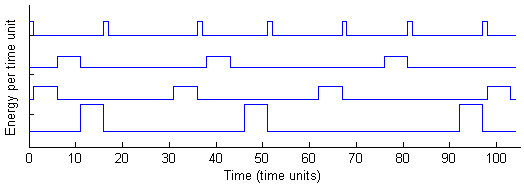
\includegraphics[scale=0.72]{edftasks.png}
\label{fig:edftasksched}
\caption{Four tasks scheduled by EDF with no smoothing.}
\end{figure}

\begin{figure}[htb]
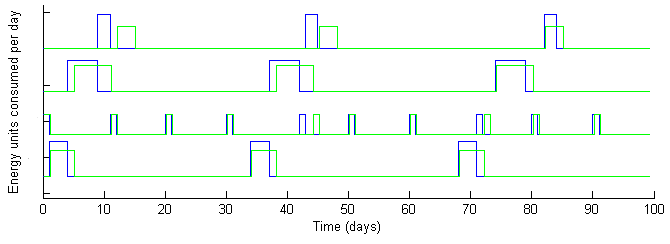
\includegraphics[scale=0.72]{stamtasks.png}
\caption{Four tasks scheduled by EDF with STAM smoothing}
\label{fig:stamtaskplot}
\end{figure}


\begin{figure}[htb]
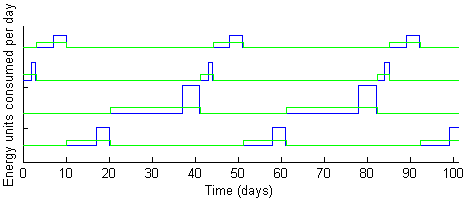
\includegraphics[scale=0.72]{stfutasks.png}
\caption{Four tasks scheduled by EDF with STFU smoothing}
\label{fig:stfutaskplot}
\end{figure}



































